%%%%%%%%%%%%%%%%%%%%%%%%%%%%%%%%%%%%%%%%%%%%%%%%%%%%%%%%%%%%%%%%%%%%%%%%%%%%%%%%
%2345678901234567890123456789012345678901234567890123456789012345678901234567890
%        1         2         3         4         5         6         7         8

\documentclass[letterpaper, 9pt, conference]{ieeeconf}  % Comment this line out if you need a4paper

%\documentclass[a4paper, 10pt, conference]{ieeeconf}      % Use this line for a4 paper

\IEEEoverridecommandlockouts                              % This command is only needed if 
                                                          % you want to use the \thanks command

\overrideIEEEmargins                                      % Needed to meet printer requirements.

% See the \addtolength command later in the file to balance the column lengths
% on the last page of the document

% The following packages can be found on http:\\www.ctan.org
%\usepackage{graphics} % for pdf, bitmapped graphics files
%\usepackage{epsfig} % for postscript graphics files
%\usepackage{mathptmx} % assumes new font selection scheme installed
%\usepackage{times} % assumes new font selection scheme installed
%\usepackage{amsmath} % assumes amsmath package installed
%\usepackage{amssymb}  % assumes amsmath package installed


\usepackage{times}
%\usepackage{natbib}
\usepackage{graphicx}
\usepackage{fixme} % This package provides a way to insert notes in draft documents
\usepackage{amsmath}
%\usepackage{multicols}
\usepackage{adjmulticol}
\usepackage{subfig}
\usepackage{url}
\usepackage{cite}

\usepackage[]{algorithm2e}
%\usepackage[]{algorithmic}

\title{\LARGE \bf
%Preparation of Papers for IEEE Sponsored Conferences \& Symposia*
Single and Dual Arm Manipulator Motion Planning Library
}


\author{Behnam Asadi$^{1}$ 
\thanks{$^{1}$Behnam Asadi is a researcher at mathematics and computer science department of university of Bremen, Germany.
        {\tt\small behnam.asadi@gmail.com}}%
\thanks{This work was supported through two grants of the German Federal Ministry of Economics and Technology (BMWi, FKZ 50 RA 1216 and FKZ 50 RA 1217 ).}
}
\begin{document}



\maketitle
\thispagestyle{empty}
\pagestyle{empty}







%\title{\LARGE \bf Constraint Based Manipulator Motion Planning}
%
%
%\author{Behnam Asadi$^{1}$ and Dr.-Ing. Jos� de Gea Fern�ndez$^{2}$% <-this % stops a space
%\thanks{Robotics Innovation Center, DFKI, Bremen, Germany}% <-this % stops a space
%\thanks{$^{1}$University of Bremen, Germany
%        {\tt\small behnam@informatik.uni-bremen.de.}}%
%\thanks{$^{2}$Dr.-Ing. Jos� de Gea Fern�ndez 
%        {\tt\small 	Jose.de_Gea_Fernandez@dfki.de }}%
%}
%
%
%\begin{document}
%
%
%
%\maketitle
%\thispagestyle{empty}
%\pagestyle{empty}


%%%%%%%%%%%%%%%%%%%%%%%%%%%%%%%%%%%%%%%%%%%%%%%%%%%%%%%%%%%%%%%%%%%%%%%%%%%%%%%%
\begin{abstract}

In this work a library for solving manipulator motion planning problems has been developed and an algorithm for imposing Cartesian constraints in single arm and dual arm operation has been proposed. The main algorithm is based on \textbf{RRT} \cite{rrt}. The code has been tested with several single arm and dual arm robots. Our method is able to find collision free paths in environments occupied with obstacles. An example of such an environment is the shelf from the Amazon picking challenge. The implemented code also enabled us to  perform complicated dual arm operations such as rotating a hand wheel or opening a drawer.
\end{abstract}
Keywords: Manipulator motion planning, dual arm operation, planning under Cartesian constraint, robotics. 

%%%%%%%%%%%%%%%%%%%%%%%%%%%%%%%%%%%%%%%%%%%%%%%%%%%%%%%%%%%%%%%%%%%%%%%%%%%%%%%%
\section{INTRODUCTION}\label{Introduction}
Nowadays, robots are no longer just machines in factory production lines and are gradually entering human everyday life and taking part in our activities. 
%On of the most important tasks in robotics, 
%and natural interaction is one of the key challenges for robots
One of the key challenges for robots is to solve motion planning problems. The task of motion planning is to find a path for moving the robot from the start state to the goal state such that the robot does not collide with itself or any other object in the environment. Various constraints including joint, torque, velocity and acceleration limits might be imposed to the task.
A classical example of motion planning is the piano mover's problem. In this problem, a piano (3D rigid object) exists in a room in the presence of some obstacles. The task is finding a path for moving the piano from start pose to the goal pose  while avoiding obstacles.
It has been shown that the piano mover's problem is PSPACE-hard \cite{reif1979complexity, Open_Motion_Planning_Library_A_Primer, LaValle:2006:PA:1213331, Latombe:1991:RMP:532147}.
%\cite{reif1979complexity}, \cite{Open_Motion_Planning_Library_A_Primer},\cite{LaValle:2006:PA:1213331} ,\cite{Choset_2005_5167} ,\cite{Latombe:1991:RMP:532147}.  
Motion planning has many applications in robotics including manipulation, autonomous cars and also in other fields such as analysis of biological molecules (protein folding), drug design and computer animation.
The rest of this paper is organized as follows: 
%In section \ref{Introduction} we introduce and  discuss the motion planning problem.
In section \ref{An Overview of Current Solutions for Motion Planning Task}, we review different approaches for solving a motion planning task. 
%In section \ref{Main Algorithm and Pipe Line for Motion Planning}, the main pipe line of the code and the third party libraries that has been used introduced.
In section \ref{Main Algorithm and Pipe Line for Motion Planning}, the main pipe line of the library is introduced.
In section \ref{Dual Arm Motion Planning},  our main algorithm for dual arm operations and our approach for imposing constraints is explained.
%We explain the library functionalities for motion planning in dynamic environment and self filtering of the robot in  section \ref{Dynamic_Environment} and \ref{Self_Filtering} respectively.
We explain the library functionalities for motion planning in dynamic environment in section \ref{Dynamic_Environment}.
Finally in section \ref{Evaluation and Experiments}, the results of our approach tested on different robots is reported. 


\section{An Overview of Current Approaches for Motion Planning Task}\label{An Overview of Current Solutions for Motion Planning Task}

%\subsection{Combinatorial Motion Planning}
%In Combinatorial motion planning, free space is decomposed into regions called cells. One popular algorithm for this purpose  is trapezoidal decomposition \cite{preparata1985computational}, \cite{seidel1991simple}. Cells with a common boundary are adjacent. An adjacency graph representing connected cells (via shared boundary ) is being created based on that. In next, the planner determines the start and the goal cells and then  searches the graph for a path connecting these two cells. The advantages of this method is that, they are complete and for problems with low dimensionality they are extremely efficient. The disadvantages are:  finding explicit representation of free space in configuration space is not a straightforward task and as the dimensionality of the configuration space increases, planning becomes impractical \cite{choset2005principles}, \cite{lavalle2006planning}.
%\subsection{Search Based}
%In this approach, the planner discretizes the work space and determines free and occupied cells. Then it generates a graph representing the planning problem and searches the graph for a solution.
%The problem with pure grid-based planning (discretizing environment and then constructing the graph) is that the sharp turns on the path do not match with the kinodynamic constraints of the robot. \textit{SBPL} \cite{sbpl} is a search based planner that uses lattice representation in which work space is discretized into a set of states with a set of motion primitives. These states are connected if there is a feasible (collision free) path between them \cite{likhachev2010search}. 
%
%Since discretization is based on motion primitives, any feasible path is dynamically compatible with the kinodynamics constraints of the robot \cite{sbpl}. 
%
%
%SBPL can search the constructed graph with the following graph search algorithms \cite{likhachev2010search}:
%\begin{itemize}
%\item Anytime dynamic  \(A* \)    \cite{likhachev2005anytime}.
%\item Anytime path planning and replanning in dynamic environments \( D* \) \cite{van2006anytime}.
%\item \(R* \): A method combining sample based planning and deterministic search \cite{likhachev2008r}.
%\end{itemize} 
%SBPL can support 2D \( (x,y) \), 3D \( (x,y, \theta) \) and N-DOF manipulator planning problems.
%Advantages of search based algorithms are their ability to incorporate various cost functions and trajectories with natural looking behaviour. The drawbacks are firstly properly discretization of configuration space (which might be a complicated task) and secondly defining a proper heuristic function.
%
%
%\subsection{Sample Based Planning}\label{Sample_Based}
%In this method, during the planning, the planner draws random samples in configuration space. If a sample is valid (i.e not in collision or any other criteria set by user) and close enough to the other generated samples (or start and goal states) it will be added to a tree. The planner continues making samples and adding them to the tree, till it can find a path from the start state to the goal state. Trees can be grown from both start and goal states (bidirectional based planner) and checking for state validation might be done when a path has been found (lazy evaluation). Some sample based algorithms are: PRM \cite{PRM} , EST \cite{EST}, RRT \cite{rrt}, SRT \cite{SRT_Plaku05sampling-basedroadmap} and their variants.
%
%The advantage of this method is robustness of planner in finding a path even in high-dimensional configuration spaces.
%On the other hand these algorithms are probabilistic and the generated path is usually jerky with redundant movements and requires smoothing and optimization.
%
%
%\subsection{Optimization Based}
%The most important issues that most of the motion planners taken into account are joint limits and obstacle avoidance while in many applications there are other criteria that should be satisfied including constraints handling, path smoothing and minimization of torque, jerk and energy consumption.
%
%
%There are other approaches that solve the motion planning problem as an optimization problem.
%\textbf{STOMP} \cite{Kalakrishnan:2011} and \textbf{CHOMP} \cite{ratliff2009chomp} are successful examples of such approaches.
%CHOMP (Covariant Hamiltonian Optimization for Motion Planning) \cite{ratliff2009chomp} is an  optimization based planning algorithm 
%in which the environment is modelled with signed distance field. The planner at first step creates  a naive initial trajectory, from the start to the goal state. Then it runs a modified version of gradient descent on a cost function which is a sum of cost of  trajectory smoothness and collision (penetration depth). Afterwards the planner tries to improve the initial path in every iteration. The advantages of this method is a smooth and natural trajectories.
%Due to the use of gradient descent, the answer might lay on a local minimum.
%
%
%STOMP (Stochastic trajectory optimization for motion planning) \cite{Kalakrishnan:2011} relies on an  optimizer that can handle cost functions that their gradients are not available. In STOMP the cost function is combination cost of colliding with obstacles (penetration depth), constraints and torque.
%The optimizer algorithm explores the space around an initial trajectory by generating a series of noisy trajectories. These trajectories  are then combined to produce an updated trajectory with lower cost.
%
%
%The advantages of this method in comparison with CHOMP are: STOMP doesn't depend on the gradient therefore is can deal with general constraints, (i.e pose or torque constraints ) and it overcomes the local minima problem of that CHOMP.
%
%
%\subsection{Potential Fields}
%In this approach the manipulator could be considered as an electric charge, the goal with the opposite charge and obstacles a potential field with the same electric charge. The obstacles will repulse the robot and the goal will attract it. This idea has been first introduced in \cite{1087247} and \cite{andrews1983impedance}.
%The advantages of potential fields is their simplicity to implement and real-time computation.
%The drawbacks are oscillations in an unstable state and trapping in local minima \cite{koren1991potential}, \cite{safadi2007local}.

%%%%%%%%%%%%%%%%%%%%%%%%%%%%%%%%%%%%%%%%%%%%%%%%%%%%%%%%%%%%%%%%%%%%%%%%%%%%%%%%%%%%%%%%%%%%%%%%%%%%%%%%%%%%%%%%%%%%%%%%%%%%%%%%%%%
Different methods have been suggested for solving a motion planning task, including combinatorial planning, search based planning, sample based planning, optimization based planning and potential fields. In combinatorial motion planning, free space is decomposed into regions called cells. One popular algorithm for this purpose  is trapezoidal decomposition \cite{preparata1985computational}, \cite{seidel1991simple}. Cells with a common boundary are adjacent. An adjacency graph representing connected cells (via shared boundary ) is being created based on that. Next, the planner determines the start and the goal cells and then  searches the graph for a path connecting these two cells. As an advantage, the approach is complete and for problems with low dimensionality it is extremely efficient. A disadvantage is that planning becomes impractical as the dimensionality of the configuration space increases \cite{choset2005principles}, \cite{lavalle2006planning}. In search based planning, the planner discretizes the work space and determines free and occupied cells. Then it generates a graph representing the planning problem and searches the graph for a solution. Several methods have been used for discretization and searching the graph including \textit{SBPL} \cite{sbpl}, \(A^* \), \( D^* \) \cite{van2006anytime} and \(R^* \) \cite{likhachev2008r}. Advantages of search based algorithms are their ability to incorporate various cost functions and trajectories with natural looking behaviour. The drawbacks are proper discretization of configuration space (which might be a complicated task) and defining an appropriate heuristic function. In sample based method, during the planning phase, the samples are drawn randomly in configuration space. If a sample is valid (i.e. no collisions or any other criteria set by the user) and close enough to the other generated samples (or start and goal states) it will be added to a tree. The planner continues making samples and adding them to the tree, until it can find a path from the start state to the goal state. Trees can be grown from both start and goal states (bidirectional based planner) and checking for state validation might be done when a path has been found (lazy evaluation). Some sample based algorithms are: PRM, EST, RRT, SRT and their variants.
%PRM \cite{PRM} , EST \cite{EST}, RRT \cite{rrt}, SRT \cite{SRT_Plaku05sampling-basedroadmap} and their variants.
Sample based planners are very robust for finding a path even in high-dimensional configuration spaces. On the other hand, these algorithms are probabilistic and the generated path is usually jerky with redundant movements and requires smoothing and optimization. A motion planning task can be seen as leading a particle in a potential field with the same electric charge towards a goal with opposite charge. The obstacles will repulse the particle (robot) and the goal will attract it. This idea has been first introduced in \cite{1087247} and \cite{andrews1983impedance}. The advantage of potential fields is their simplicity to implement and real-time computation. The drawbacks are oscillations in an unstable state and trapping in local minima \cite{koren1991potential}, \cite{safadi2007local}. The most important issues that most of the motion planners have taken into account are joint limits and obstacle avoidance while in many applications there are other criteria that should be satisfied including constraints handling, path smoothing and minimization of torque, jerk and energy consumption. In optimization based planning, the planner defines a cost function in which the cost is weighted according to collision, path length, path smoothness, energy consumption and joint/ torque limits. Then the planner tries to reduce the cost by calling an optimizer over the generated path. In CHOMP (Covariant Hamiltonian Optimization for Motion Planning) \cite{ratliff2009chomp}  the environment is modelled with signed distance field. The planner at first step creates  a naive initial trajectory, from the start to the goal state. Then it runs a modified version of gradient descent on a cost function which is a sum of cost of trajectory smoothness and collision with obstacles (penetration depth). Afterwards the planner tries to improve the initial path in every iteration. The advantages of this method is a smooth and natural looking trajectory. Due to the use of gradient descent, the answer might lay on a local minimum. STOMP (Stochastic trajectory optimization for motion planning) \cite{Kalakrishnan:2011} relies on an optimizer that can handle cost functions where their gradients are not available. In STOMP the cost function is the combination cost of colliding with obstacles (penetration depth), constraints and torque.
The optimizer algorithm explores the space around an initial trajectory by generating a series of noisy trajectories. These trajectories  are then combined to produce an updated trajectory with lower cost. Since the STOMP doesn't depend on gradients, it can deal with general constraints (i.e. pose or torque constraints) and it overcomes the local minima problem of the CHOMP.
%%%%%%%%%%%%%%%%%%%%%%%%%%%%%%%%%%%%%%%%%%%%%%%%%%%%%%%%%%%%%%%%%%%%%%%%%%%%%%%%%%%%%%%%%%%%%%%%%%%%%%%%%%%%%%%%%%%%%%%%%%%%%%%%%%%%
\section{Main Algorithm and Pipe Line for Motion Planning}\label{Main Algorithm and Pipe Line for Motion Planning}
We have created our sample based motion planning library based on \textbf{OMPL} \cite{sucan2012the-open-motion-planning-library} and we have been mainly inspired by  \textbf{MoveIt!} \cite{6377468}, \cite{moveit} for the main pipeline and architecture, however we have added support for dual arm operation, imposing Cartesian constraints, self filtering and planning in a dynamic environment.


OMPL is an open source motion planning library that covers most of the state of the art sample based motion planning algorithms and MoveIt! is software for mobile manipulation including tools for 3D perception, collision checking, solving inverse and forward kinematics queries and control of the robot.

Due to the dependency of MoveIt! on the ROS framework, it was not possible to integrate it with our robotic framework,  \textit{ROCK}
\footnote{http://rock-robotics.org}.

As it has been briefly discussed in section \ref{An Overview of Current Solutions for Motion Planning Task}, sample based motion planners generate random states in configuration space. Then by applying forward kinematics, we check the validity of the state  (self collision and collision with environment). In the case of validity of the newly drawn sample, it will be added to the RRT. This process continues until a path between start and goal configuration can be found or some termination condition are met (i.e planning time  exceeds maximum allowed time).

%As it has been briefly discussed in \ref{Sample_Based}, the \textbf{OMPL} motion planner generate a random state (depending on the configuration in Cartesian space or joint space). The by applying forward kinematic(if planning is joint space) or inverse kinematics (if planning is Cartesian space), we check the state validity by checking joint limits,  self collision and collision with environment. In the case of validity the newly drawn sample will be added to the RRT tree. This process continues until a path between start and goal configuration can be found.


%\subsubsection{Planning Under Cartesian Constraint}



\subsection{IK Solver With Minimum Movements and Jerk for High Degree of Freedom}\label{IK_Solver_With_Minimum_Movements_and_Jerk_for_High_Degree_of_Freedom}
One of the most important parts of the motion planning problem is solving inverse kinematic queries. Two main approaches for solving inverse kinematic problems are numerical solutions and analytical (closed form) solutions.


\textit{KDL} \cite{smits2011kdl} (Kinematics and Dynamics Library)\footnote{http://www.orocos.org/kdl} is a library for computing forward and inverse kinematic queries with numerical solutions. 
Due to recursive nature of numerical solutions for solving IK problems, they might be very slow or trap in local maxima.
%Analytical (closed form) solutions are another method for solving forward and inverse kinematic request. 
\textit{Openrave}  (Open Robotics Automation Virtual Environment ) \cite{Diankov_2008_6117}  is a software for simulating and deploying planning algorithm. It provides a tool called \textit{IKFast} which can generate  \textit{C++} code (independent of any library) representing the model of the manipulator for solving forward and inverse kinematic queries. The generated code is able to solve  the request on the order of 4 microseconds \cite{ik_fast_doc}.


One key issue with using IKFast for solving IK queries is finding proper values for manipulators free joints (redundant joints). Furthermore, we would like to have a hierarchical structure for free joints such that the joints that are closer to the root of kinematic chain have less movements relative to those that are closer to end effector. The motivation for such a decision is that we like to have minimum movements and jerk during the manipulation.
%The reason for such a decision is to minimize the movement. 
For instance, consider a kinematic chain in a humanoid robot from knee  to the right (or left) wrist. In the case we want to use this kinematic chain for grasping an object, we like to use the joints in the lower part less (in torso or knee) and use more joints in the arm.


To overcome this issue, we discretize the space between the upper and lower joint limits for every free joint and search for possible values starting from either a given configuration (configuration specified by user or from the IK solution of the previous Cartesian way point in the trajectory or the middle point between joint lower and upper bound).
% till we find a solution. 
This starting point policy is very crucial since starting from joint lower limit and checking values for solution toward upper limit will bias the IK solution to the joint limits, specially when there is more than one free joint in the chain. The code has been implemented recursively so it is capable of handling arbitrary number of free joints. Algorithm \ref{alg:IK_solver_algorithm_for_free_joint_parameter} describes the recursive function for finding free joints parameter.




\begin{algorithm}
\SetKwData{Left}{left}
\SetKwData{This}{this}
\SetKwData{Up}{up}
\SetKwFunction{Union}{Union}
\SetKwFunction{FindCompress}{FindCompress}
\SetKwInOut{Input}{Input}
\SetKwInOut{Output}{Output}
\caption{Algorithm for finding free joint parameter for IK queries with IKFast.}
%\caption{disjoint decomposition}
\Input{Robot model, Vector of free joints, Cartesian pose}
\Output{Values for free joint, IK solution}

Recursive\_free\_joints\_value (values\_for\_free\_joints\_vector, index)

    \eIf{($index>0$)}
    {
           \While{$\left( \text{joint lower bound} < pivot+step \right) $ $||$ $\left( pivot+step< \text{joint upper bound} \right)$ }
            {
                step\gets step+step\_size 
               
                    values\_for\_free\_joints\_vector.push\_back(pivot+step) \par
                    \If{ recursive\_free\_joints\_value (values\_for\_free\_joints\_vector, index-1) }
                    {
                        return true \par
                    }
                    values\_for\_free\_joints\_vector.pop\_back() \par
                    values\_for\_free\_joints\_vector.push\_back(pivot-step) \par
                    \If{ recursive\_free\_joints\_value( values\_for\_free\_joints, index-1)}
                    {
                        return true \par
                    }
                    values\_for\_free\_joints\_vector.pop\_back() \par
             }
    }
    {
		\While{$\left( \text{joint lower bound} < pivot+step \right)$ $||$ $\left( pivot+step< \text{joint upper bound} \right)$ }
		{

			step \gets step+step\_size\;\dosemic
			
			\If {IKFast(Cartesian pose,values\_for\_free\_joints\_vector, pivot+step, index)$||$ IKFast(Cartesian pose,values\_for\_free\_joints\_vector, pivot-step, index)}
			{
				return true \par
			}
		
		}
    }
    return false  \newline

\label{alg:IK_solver_algorithm_for_free_joint_parameter}
\end{algorithm}










\section{Motion Planning Under Cartesian Constraints}\label{Motion_Planning_under_constraints}





Motion planning tasks always come with various constraints. These constraints make some states impermissible for the robot.
Primitive examples of such constraints are collision avoidance and joint limits.

In many manipulation tasks some other constraints should also imposed on the robot to satisfy the problem conditions.
Examples of these are constraints on the orientation of the end effector or on the X,Y,Z Axis of the end effector.

Various solutions proposed by researchers for imposing constraints on EEF in \cite{stilman2007task, Koga:1994:PMI:192161.192266, bertram2006integrated, drumwright2006toward}. These algorithms are either not efficient or developed for a specific constraint representation\cite{berenson2011task}.
The authors in CBiRRT\cite{berenson2010probabilistically} developed a framework for imposing constraints represented by TSRs (task space regions).
The algorithm has a constraint satisfaction strategy (projection/ rejection) and general planning algorithm (sample based planner).
%The solutions used from control theory for enforcing constraint are either use gradient descent method which has the local minimum problem or use dynamic programming which is not efficient in configuration space with high dimensionality. 
CBiRRT employs the robustness of RRT planners to explore the configuration space and enforce samples with projection/ rejection policy based on gradient decent\cite{berenson2011task}.




In the motion planning library that we developed, we add the capability of setting Cartesian constraints for single arm and dual arm tasks.
The main algorithm for motion planning under constraints is RRT based. 
The planner always checks if any constraints have been set during the initialization of planner.
In the case a constraint has been set, the planner will change the sampling space from joint space to Cartesian space and it plans for the manipulated object. In other words, the drawn sample represents the object position. The samples are drawn within the upper and lower bound of imposed constraint to satisfy the task requirements. The Cartesian constraint which are imposed to the planner are similar to TSRs in CBiRR. By having the grasp pose for the object and object pose, the end effector pose for the arm can be determined. Afterwards, we search for a valid inverse kinematic solution (by taking into account joints limit, self collision and collisions with environment). 
%In the case of a valid one found,
When a valid solution is found, it will be added to the RRT. If the planner can find a path between start and goal pose within the time limit for planning (or before the maximum number of iteration reaches), the trajectory will be published. 
%Figure \ref{The-Motion-Planning-Pipeline-Cartesian-Space} illustrates the flow chart of our algorithm.

%\begin{minipage}{0.47\textwidth}\end{minipage}

\begin{algorithm}
\SetKwData{Left}{left}
\SetKwData{This}{this}
\SetKwData{Up}{up}
\SetKwFunction{Union}{Union}
\SetKwFunction{FindCompress}{FindCompress}
\SetKwInOut{Input}{Input}
\SetKwInOut{Output}{Output}
%\caption{disjoint decomposition}
\Input{Robot model, motion planning request, Cartesian Constraint}
\Output{Collision free trajectory}
	\While{Time has left for planning}
	{
		Draw a random sample from Cartesian space Between upper and lower constraint limits\;
		\eIf{There is IK solution for the drawn sample}
		{
  				Update the robot state with IK Solution \newline
  				\uIf{robot is in self collision state}
  				{
  				
					\If{Collisions are not in the allowed collisions list}
					{
						next 				
					}  				
  				
  				}\uElseIf{robot is not in Collision with the environment}
  				{
  					Add the newly drawn sample to the RRT
  				}
 		}
 		{
			next		
 		}
 		\If{There is a valid path between start and goal in RRT}
 		{
			publish the path \newline			
			return	
 		}
 	}
\caption{Motion planning under Cartesian constraints algorithm}
\label{alg:Motion_planning_under_Cartesian_constraints_algorithm}
\end{algorithm}


\section{Dual Arm Motion Planning}\label{Dual Arm Motion Planning}
%realm of robotic 
While in the domain of robotics, manipulation can be interpreted as an interaction with an object, dual arm manipulation doesn't have a common and general accepted definition \cite{Smith20121340}.
"In fact, many authors do not distinguish between multi-agent or multi-arm systems" \cite{Smith20121340}.
Employing two arms for manipulation has several advantageous. Using two arms gives the robot more strength (loading a heavy object for example) and for the tasks that are initially designed for human, it gives robot better dexterity compared to one arm \cite{Smith20121340}.


The Authors in \cite{5686273}, classified dual arm operation into \textbf{non-coordinated manipulation}, where each arm is doing separated motions (manipulating an object with one arm while moving another object with a second arm for instance), and \textbf{coordinated manipulation} (opening a bottle of wine for example), in which the arms are working on the same task. Coordinated manipulation can be subdivided into \textbf{goal-coordinated} (playing piano, typing with keyboard) and \textbf{bimanual} manipulation.

In goal-oriented manipulation, in which both arms are solving the same task, the arms are not physically interacting with each other. In bimanual operations motion of one arm is widely based on motions of the other one which might be \textit{symmetric, asymmetric, congruent or non-congruent} \cite{5686273}.


In this work, we have designed three scenarios for performing  dual arm operations which requires bimanual manipulation. We have achieved planning for these tasks by using same code and only changing the parameters of imposed constraints.
The first task is rotating a hand wheel, the second one is opening/closing a drawer and the third one is moving an object with both arms while keeping the orientation. The interaction between EFFs and hand wheel/ drawer is performed via a grasping component which is based on vision and force control, developed by DFKI \footnote{http://robotik.dfki-bremen.de/en/startpage.html} research center.

\begin{algorithm}
\SetKwData{Left}{left}
\SetKwData{This}{this}
\SetKwData{Up}{up}
\SetKwFunction{Union}{Union}
\SetKwFunction{FindCompress}{FindCompress}
\SetKwInOut{Input}{Input}
\SetKwInOut{Output}{Output}
%\caption{disjoint decomposition}
\Input{Robot model, motion planning request, Cartesian Constraint}
\Output{Dual arm collision free trajectory}
	\While{Time has left for planning}
	{
		Draw a random sample representing object from Cartesian space Between upper and lower constraint limits\;
		\eIf{There is IK solution for the drawn sample for the first arm}
		{
  				Update the robot state with IK Solution\;
  				\If {There is IK solution for the second arm from updated robot state}
  				{
  					\uIf{robot is in self collision state}
  					{
						\If{Collisions are not in the allowed collisions list}
						{
							next					
						}  				
  				
  					}\uElseIf{robot is not in Collision with the environment}
  					{
  						Add the newly drawn sample to the RRT.
  					}  					
  				}		
 		}
 		{
			next
 		}
 		\If{There is a valid path between start and goal in RRT}
 		{
			publish the path
			return
 		}
 	}
\caption{Dual Arm Motion Planning algorithm}
\end{algorithm}



\subsection{Pre-Scripted vs Constraint Task}
In order to perform some dual arm operations, which requires imposing constraints (for example carrying a glass of water while keeping the orientation or opening a drawer with both arms) we have examined two different approaches:
\begin{itemize}
\item \textbf{Pre-scripted planning}
\item \textbf{Constrained based planning}
\end{itemize} 

In the pre-scripted approach, at first a Cartesian path consisting of way points (for example a half circle in the case of rotating a hand wheel or a straight line in the case of opening a drawer which represent the  end effector path) is being calculated. Then by calling the IK solver, the corresponding joint values are retrieved. Generalizing tasks with pre-scripted approaches requires calculating and rewriting new way points for new tasks which limits the functionality of the code. In the constraint based approach, after specifying the start and the goal pose, we can define constraints on X,Y,Z axis and orientation (roll, pitch, yaw) of the object frame. By changing the values of the parameters, it is possible to reuse the code for different task.
\subsection{Constraint Based Dual Arm Motion Planning Algorithm}
The algorithm for dual arm motion planning under constraints is similar to the approach that was introduced in section \ref{Motion_Planning_under_constraints}, except that the kienmatic reachability is checked for both arms. 
\section{Dynamic Environment}\label{Dynamic_Environment}
During a motion planning task, the robot senses the environment via its sensors and after finding a path, it executes the trajectory.
In many situations, the state of the environment during the execution of the trajectory might change, therefore following the computed trajectory might cause collision. Various approaches have been proposed for modelling obstacles in dynamic environments (completely unpredictable obstacles, partial predictable obstacle) with different strategies for planning (probabilistic models, bounded uncertainty models, game theoretic models and dynamic replanning) \cite{ICRA_2012_Tutorial}.
In a methd called "Time-bounded lattice for planning in dynamic environments" \cite{kushleyev2009time}, the algorithm tries to predict the position of dynamic obstacles by modelling their trajectories. Then it uses a time-bounded lattice (a short-term planning in time with longterm planning without time) for planning and obstacle avoidance.
%In \cite{Motion_Strategies_for_People_Tracking_in_Cluttered_and_Dynamic_Environments}
In some problems, the pose of the obstacles might be dependent on the pose of the robot (i.e non cooperative game with two players). For solving such problems, models from game theory have been used. In \cite{ruiz2012homicidal}, the author solved the  the problem of capturing an omnidirectional evader using a DDR (differential drive robot) by employing such models.
The algorithms in \cite{likhachev2009planning} and \cite{fiorini1998motion} try to compute an appropriate velocity for the robot such that it dodges  obstacles in a short time step. The \( D^* \) \cite{van2006anytime} algorithm can handle the dynamic obstacles found during the execution of the trajectory so it can be used in unpredictable environments. The algorithm in \cite{park2013real}, combines replanning algorithms with optimization-based planning to handle dynamic obstacles. The algorithm utilizes the parallelization on multi GPUs to  optimizes multiple trajectories to generate a high-quality path.
Here in this work since our main focus was not planning in dynamic environments, we have used a simple yet workable approach. The planner checks the validity of each state in the trajectory during execution of that trajectory. If some states are broken, the planner will try to find a collision free path right before and after the broken state (replanning only over the invalid states and not whole the path) and update the trajectory. 
%Depending on the way we model the environment, the obstacles could be traceable or the environment could be completely unpredictable. 
%Various approach has been proposed for solving the problem of planning in dynamic environment.
\begin{algorithm}
\SetKwData{Left}{left}
\SetKwData{This}{this}
\SetKwData{Up}{up}
\SetKwFunction{Union}{Union}
\SetKwFunction{FindCompress}{FindCompress}
\SetKwInOut{Input}{Input}
\SetKwInOut{Output}{Output}
%\caption{disjoint decomposition}
\Input{Robot model, motion planning request,robot environment point cloud, initial trajectory}
\Output{Updated collision free trajectory}


	\While{execution of trajectory is not finished}
	{
		%read joint angles, update robot state with read joint angles\;
		%update robot collision checker with acquired OctoMap, check the validity of each state in trajectory \;
		read the trajectory from the planner
		obtain the point cloud from sensors, create OctoMap from point cloud
		update robot collision checker with acquired OctoMap
		\For{every state in the trajectory} 
		{
			check the validity of state and mark down invalid states
		}	  
 
		\For{every invalid state in the trajectory} 
		{
			start state $\gets $ state right before the invalid state
			goal state $\gets $  state right after invalid  state
			call the planner for planning between start and goal state
			\eIf{planning succeed}
  			{
  				update initial trajectory with newly computed trajectory
  			}
  			{
	  			cancel the execution of trajectory
	  			return false
  			}
		}	  
 	}
\caption{Replanning in dynamic environment algorithms.}
\end{algorithm}



  

%\section{Self Filtering}\label{Self_Filtering}
%One problem that a robot might face during the planning is that it might sense itself (or part of itself) via 3D scanner and add the acquired data as occupied zone and consequently, robot will find itself in a permanent collision state. 
%For solving this problem, we have added a functionality to our library for self filtering.
%By computing the forward kinematic from the current joint state, we compute the pose of URDF \footnote{http://wiki.ros.org/urdf} link and URDF visuals. Then we fit the robot visual into a convex hull polygon and subtract that from the incoming data of the 3D scanner. The result is the sensed scene without the robot in it. 

\section{Evaluation and Experiments}\label{Evaluation and Experiments}
To evaluate the robustness and performance of our planner, we have tested the planner on several robots with 6, 7 and 11 DOF for single arm and dual arm operation.
We also designed several scenarios and experiments to check the success rate and recorded the required time for planning in a simulation environment. 
These experiment have been done on a PC with 64-bit architecture equipped with Intel Core i7-3770 CPU (3.40GHz) and 7.5 GiB of ram. 
\subsection{AILA}\label{AILA}
The robot AILA \cite{5979775}, is a dual arm mobile robot developed at DFKI \footnote{http://robotik.dfki-bremen.de/en/startpage.html} research center with a total of 70 degrees of freedom: 2 x 7-DOF arms, 4-DOF torso, 2-DOF head, 12-DOF mobile base, 2 x 18-DOF hands. We defined several planning groups including right arm, left arm and right arm plus foot, knees and torso.
The combination of the two latter groups, make a bigger planning group with the form of a tree which gives more flexibility for dual arm operations. In the following we describe the experiments and outcomes.
\subsubsection{Bookshelf desk}\label{Bookshelf_Desk}
In this task the planner will try to place the right arm of the AILA in the middle of a bookshelf desk.
We examined different planners with the maximum time limit of 10 seconds for planning. Note that required time for the whole task is more than 10 seconds (i.e path smoothing, interpolation, IK solving). 
Figures \ref{aila_box_plot_bookshelf_desk} and \ref{aila_success_chart_bookshelf_desk} show the box plot and success rate of different planners.
\begin{figure}
\centering
\subfloat[]
{
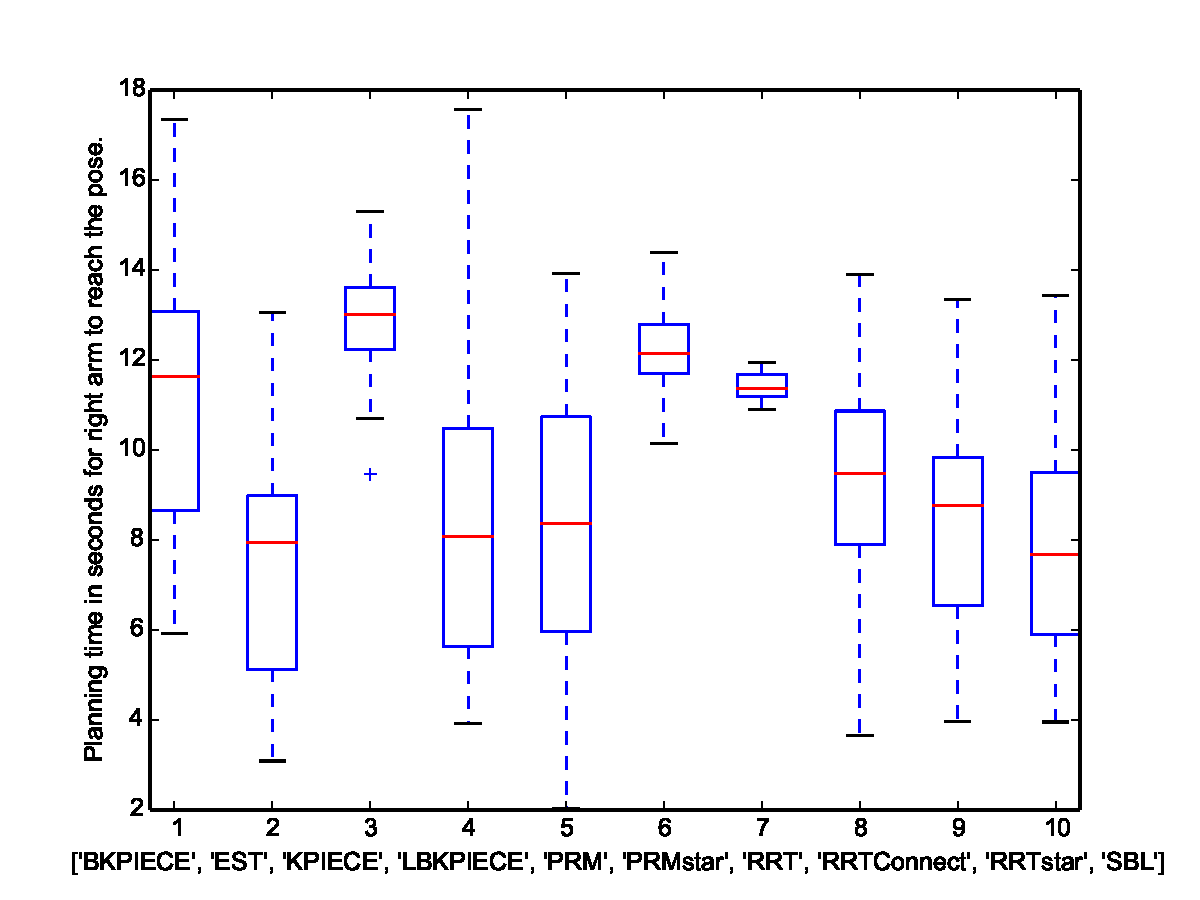
\includegraphics[width=0.45\textwidth]{figures/Aila/planners_execution_time_shelfbook_aila.pdf}
}
\caption{The box plot of planning time for accessing middle point of a book shelf with different planners.}
\label{aila_box_plot_bookshelf_desk}
\subfloat[]
{
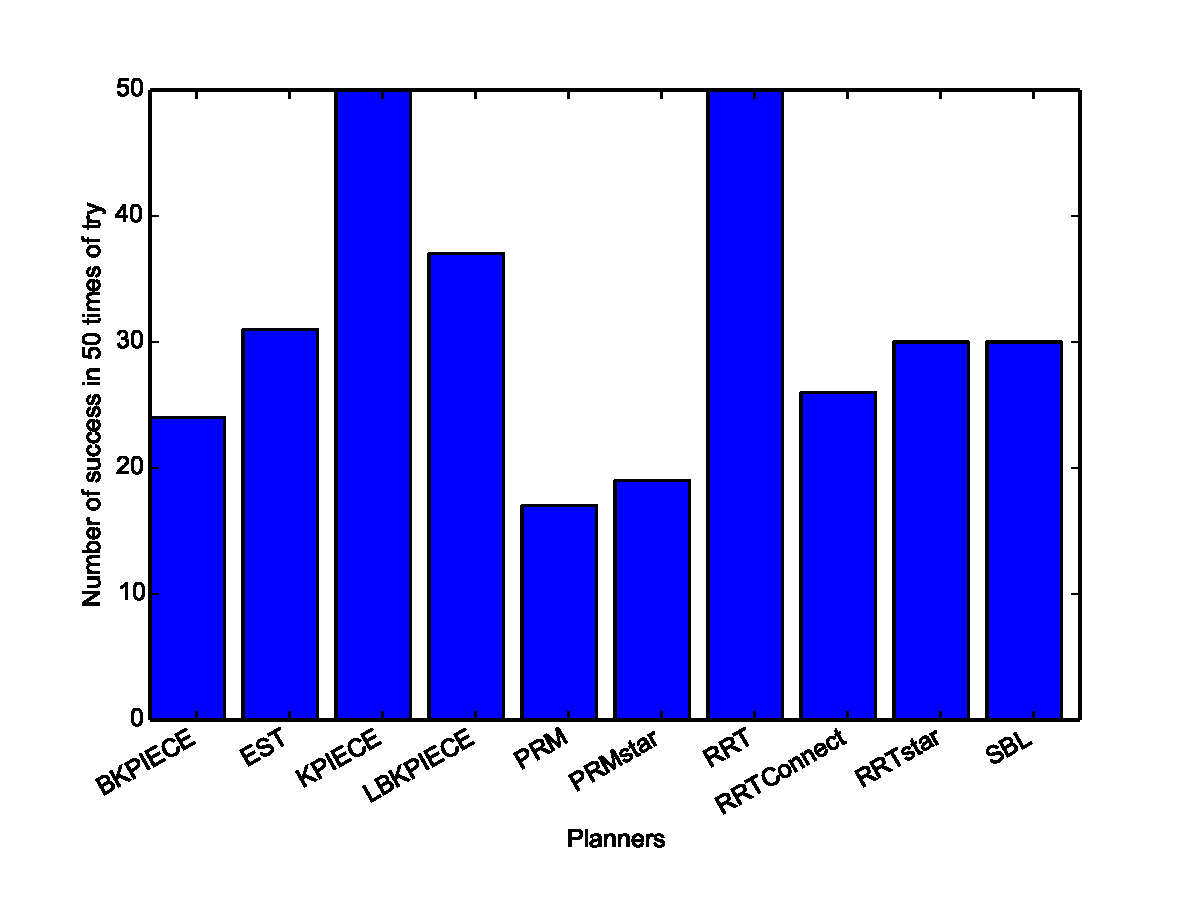
\includegraphics[width=0.45\textwidth]{figures/Aila/planners_success_rate_shelfbook_environment_AILA.pdf}
}
\caption{Success rate of different planners to access book shelf within 50 times of trial.}
\label{aila_success_chart_bookshelf_desk}
\end{figure}


\subsubsection{Amazon Picking Challenge }
For this task, first robot places itself in front of the shelf by using its mobile base, such that the base link of the robot is in the middle of the shelf columns that needs to be reached. Then the planner will try to find a collision free path to place the right arm in the shelves from A to L. For this task we haven't set any time limits for planning. Figures \ref{aila_box_plot_bookshelf_desk_amazon_pickin_up_number_of_states}  and \ref{aila_box_plot_bookshelf_desk_amazon_pickin_up_planning_time} show the the box plot of required time for finding collision free trajectory from the start pose to the shelves B,E,H,K.

%\footnote{http://icra2015.org/conference/robot-challenges#!amazon_pick_banner_robot}


\begin{figure}
\centering
\subfloat[]
{
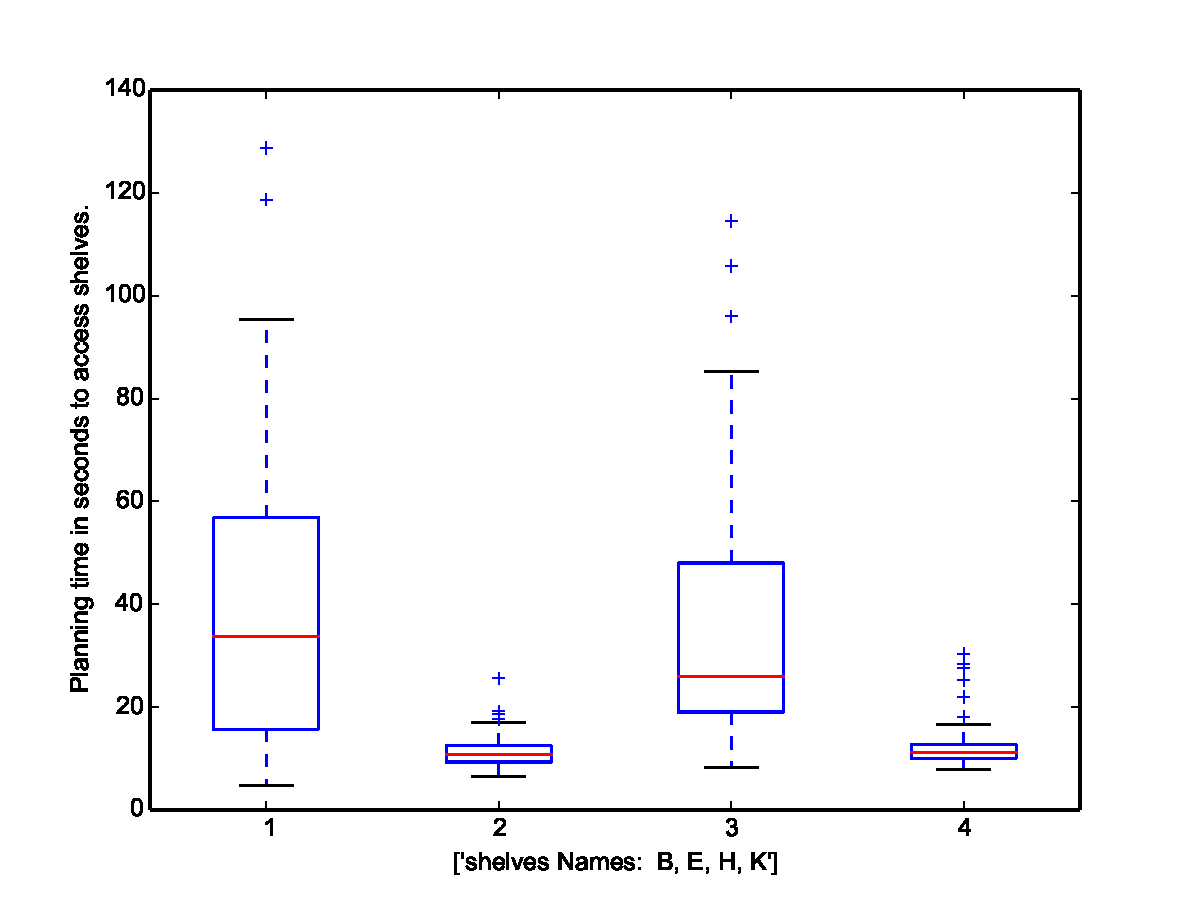
\includegraphics[width=0.45\textwidth]{figures/Aila/planners_execution_time_shelfbook_aila_amazon_picking_up.pdf}
}
\caption{The box plot of planning time for the shelves B,E,H,K of Amazon picking challenge.}
%\caption{}
\label{aila_box_plot_bookshelf_desk_amazon_pickin_up_planning_time}
\subfloat[]
{
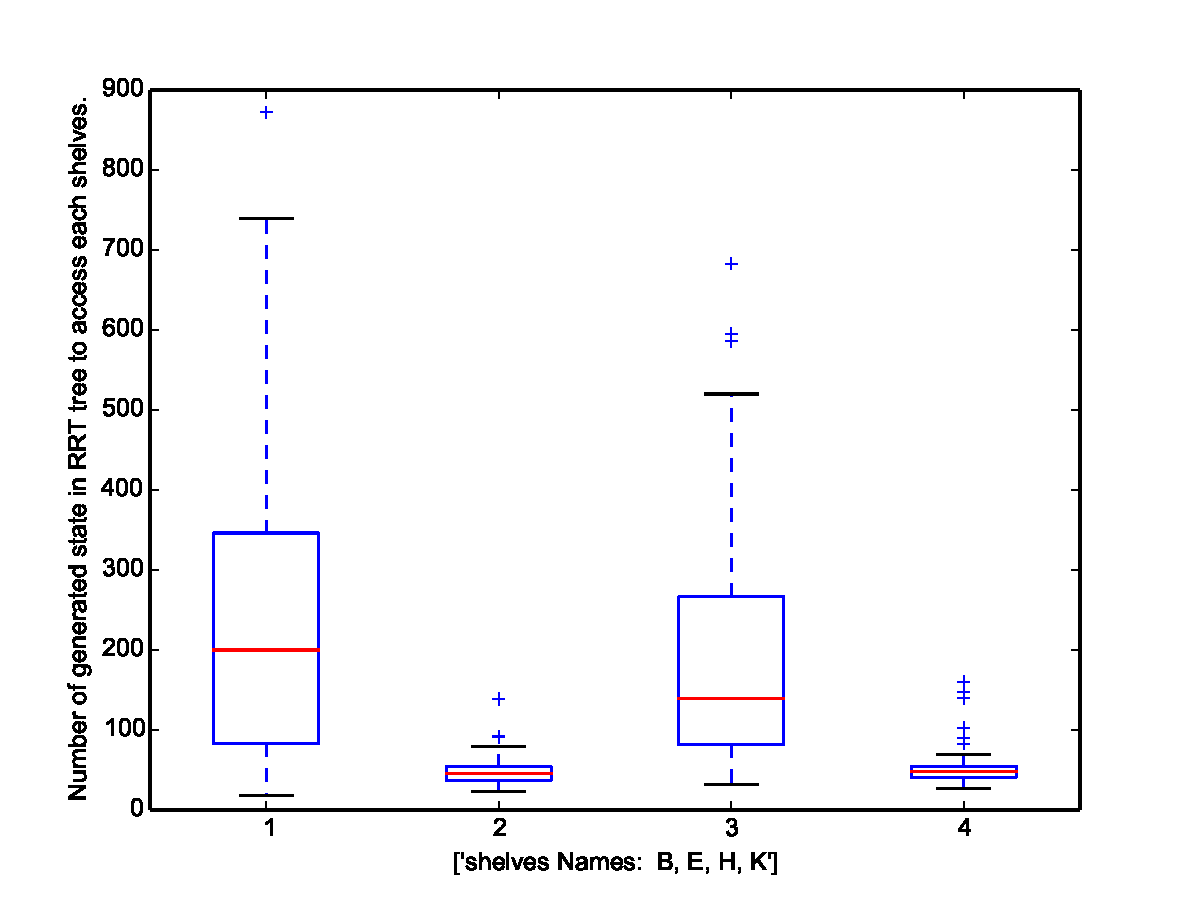
\includegraphics[width=0.45\textwidth]{figures/Aila/Number_of_generated_state_in_RRT_tree_to_access_each_shelves_aila_amazon_picking_up.pdf}
}
\caption{The box plot of total number of generated state in RRT for accessing each shelf of Amazon picking challenge.}
\label{aila_box_plot_bookshelf_desk_amazon_pickin_up_number_of_states}
\end{figure}





 
%\subsubsection{Dual Arm Carrying Objects under Cartesian Constraint}
%By imposing proper constrain on the algorithm introduced in \ref{Motion_Planning_under_constraints} it is possible to perform dual arm tasks which requires constrain. Example of  such tasks are opening drawer, turning hand wheel or moving an object with two arm while keeping orientation.
%Here we have examined the task of dual arm moving an object from one level of shelf to the other level.



\subsection{ARTEMIS}
The ARTEMIS\footnote{http://robotik.dfki-bremen.de/de/forschung/robotersysteme/artemis.html.} robot developed by DFKI, consists of a rover with 6 wheels and 6-DOF manipulator mounted on top of the rover. We examined the task of carrying an object while keeping the orientation of the EFF from one side of robot to the other side. The task achieved by using the algorithm explained in section \ref{Motion_Planning_under_constraints}. Figure \ref{semprom_artemis_constraint} illustrates ARTEMIS arm carrying an object while keeping the orientation.


\subsection{SemProM}

The dual arm SemProM-Robot\footnote{http://robotik.dfki-bremen.de/en/research/robot-systems/mr-semprom-1.html.} which is the predecessor of AILA, designed for controlling, transportation and gripping of objects.
The robot consists of two 7-DOF schunk lwa, a flexible head and a base frame. 
%This anthropomorphous design is resumed in the head where the control units of the robot is located.
Here we completed the task of opening a hand wheel and opening (pulling) a drawer by imposing different constraints and the algorithm explained earlier in section
\ref{Motion_Planning_under_constraints}. For example, in order to open a hand wheel, it should rotate $\pi/2$  over its \textbf{x} axis. By imposing the  constraints in equation \ref{eq:opening_hand_wheel} , the robot was able to open a hand wheel.

For the task of opening a drawer, since the only desired movement is in the \textbf{y} axis, simply by setting the constraints on \textbf{y} and no rotations the task could be accomplished. equation \ref{eq:opening_hand_drawer} represents such a constraint. 


 

\begin{equation}
\begin{pmatrix}
x: 0.70\\ 
y: 0.00 \\  
z: 0.00\\ 
roll:  \pi/2\\  
pitch: 0.0\\ 
yaw: 0.0
  \end{pmatrix}
, \ \  
  \begin{pmatrix}
	x: 0.70\\  
	y: 0.00\\ 
	z: 0.00\\
	roll: 0.0\\  
	pitch: 0.0\\ 
	yaw: 0.0   
  \end{pmatrix}
\label{eq:opening_hand_wheel}
%\text{Upper and lower bound of Cartesian constraint for opening a hand wheel.}
\end{equation}  









\begin{equation}
\begin{pmatrix}
  x: 0.0\\ 
  y: 1.00\\ 
  z: 0.00\\ 
  roll: 0.0\\  
  pitch: 0.0\\ 
  yaw: 0.0
  \end{pmatrix}
, \ \  
  \begin{pmatrix}
	x: 0.0\\  
	y: -1.00\\  
	z: 0.00\\ 
	roll: 0.0\\  
	pitch: 0.0\\ 
	yaw: 0.0 
  \end{pmatrix}
\label{eq:opening_hand_drawer}  
\end{equation}  



 
Figure \ref{semprom_artemis_constraint} illustrates opening a hand wheel by imposing constraints with \textbf{Mr Semprom}.
\begin{figure*}
\centering
\subfloat[]
{
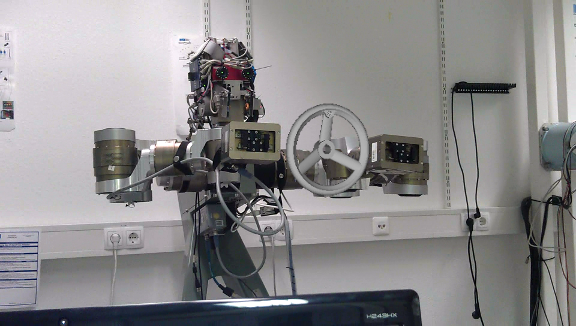
\includegraphics[width=0.30\textwidth]{figures/MrSemprom/vlcsnap-2015-01-22-11h13m13s40.png}
}
\subfloat[]
{
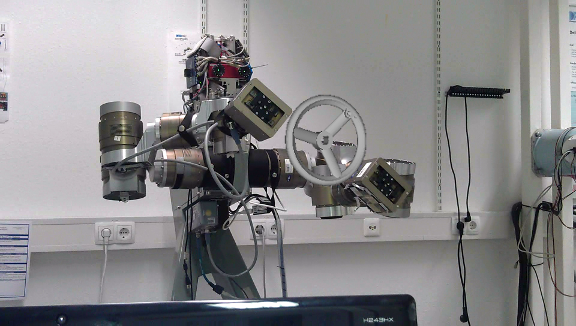
\includegraphics[width=0.30\textwidth]{figures/MrSemprom/vlcsnap-2015-01-22-11h09m10s174.png}
}
\subfloat[]
{
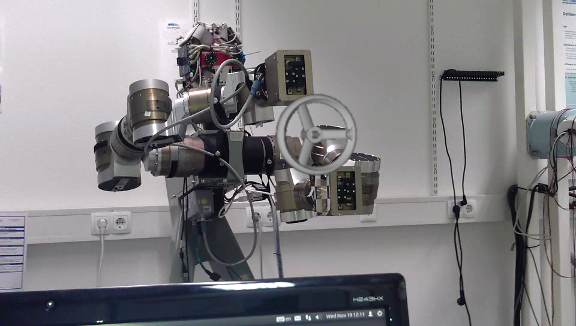
\includegraphics[width=0.30\textwidth]{figures/MrSemprom/vlcsnap-2015-01-22-11h08m47s170.png}
}


\subfloat[]
{
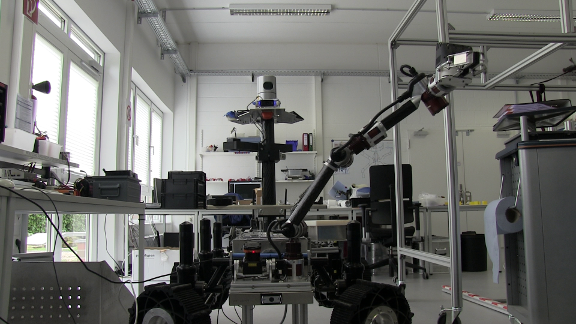
\includegraphics[width=0.30\textwidth]{figures/ARTEMIS/vlcsnap-2015-06-03-16h28m10s8.png}
}
\subfloat[]
{
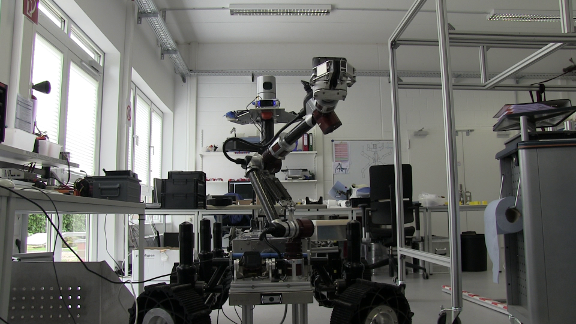
\includegraphics[width=0.30\textwidth]{figures/ARTEMIS/vlcsnap-2015-06-03-16h28m32s62.png}
}
\subfloat[]
{
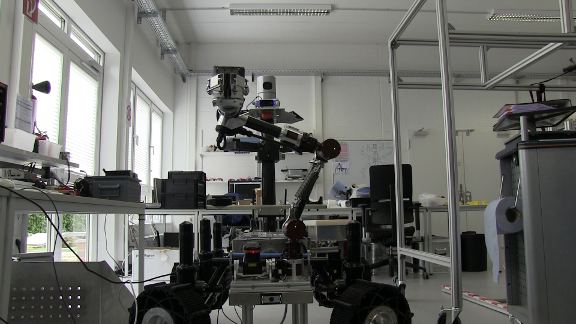
\includegraphics[width=0.30\textwidth]{figures/ARTEMIS/vlcsnap-2015-06-03-16h29m00s77.png}
}
\caption{The robot SemProM (on the top) rotates a hand wheel, the robot ARTEMIS (on the bottom) carries an object while keeping the orientation. The tasked achieved by employing the algorithm \ref{alg:Motion_planning_under_Cartesian_constraints_algorithm} and the constraints from equation \ref{eq:opening_hand_wheel} and \ref{eq:opening_hand_drawer}.}
\label{semprom_artemis_constraint}
\end{figure*}
\begin{figure*}
\centering
\subfloat[]
{
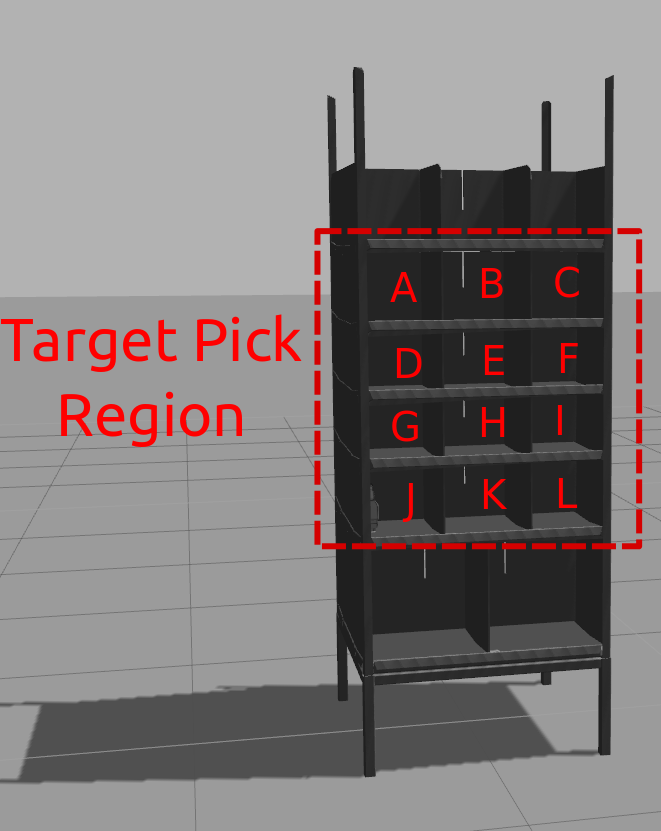
\includegraphics[width=0.25\textwidth]{figures/Aila/gazebo_pod3.png}
}
%\subfloat[]
%{
%\includegraphics[width=0.30\textwidth]{figures/Aila/vlcsnap-2015-06-04-16h33m21s54.png}
%}
%\subfloat[]
%{
%\includegraphics[width=0.30\textwidth]{figures/Aila/vlcsnap-2015-06-04-16h34m09s95.png}
%}
\subfloat[]
{
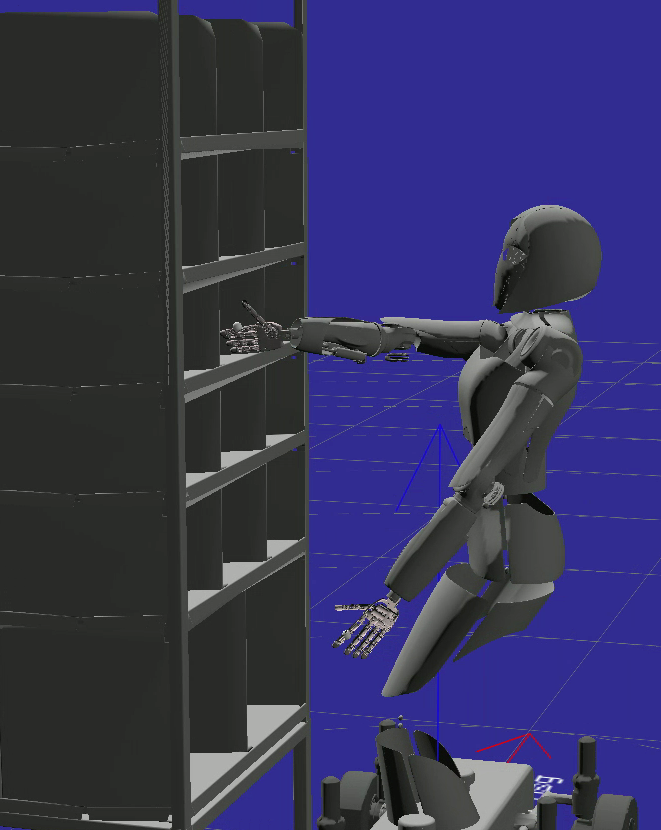
\includegraphics[width=0.25\textwidth]{figures/Aila/vlcsnap-2015-06-04-16h34m17s175.png}
}
%\subfloat[]
%{
%\includegraphics[width=0.30\textwidth]{figures/Aila/vlcsnap-2015-06-04-16h35m01s108.png}
%}
\subfloat[]
{
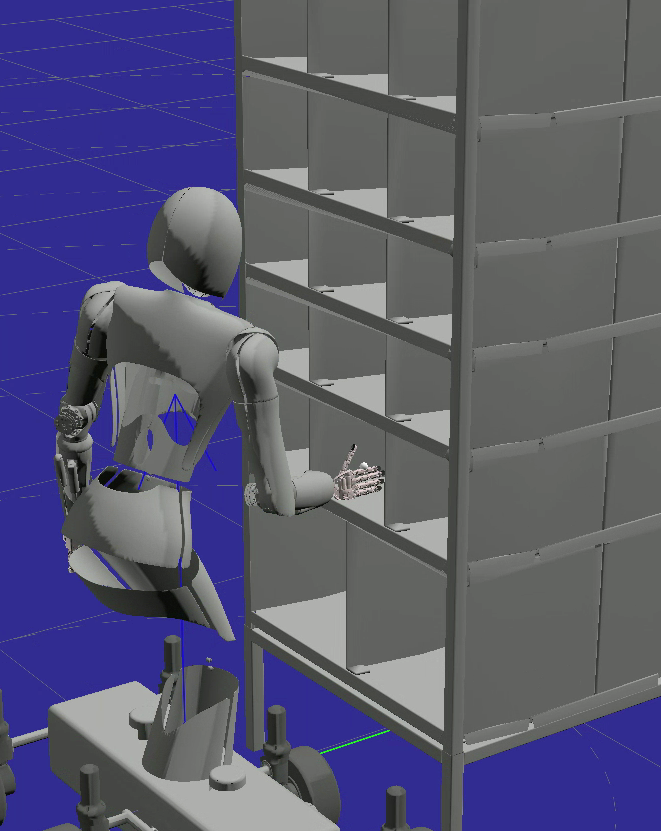
\includegraphics[width=0.25\textwidth]{figures/Aila/vlcsnap-2015-06-04-16h36m01s205.png}
}
\caption{The robot AILA access the shelves B,E,H,K form  "Amazon Picking Challenge Shelf" respectively.}
\label{aila_amazon_picking_up}
\end{figure*}



%%%%%%%%%%%%%%%%%%%%%%%%%%%%%%%%%%%%%%%%%%%%%%%%%%%%%%%%%%%%%%%%%%%%%%%%%%%%%%%%
%\section{Results Analysis and Conclusion}

\section{Analysis and Conclusion}
One common parameter in all RRT based planers is "range". Range is the threshold at which, newly drawn samples with smaller distance value than that (distance  to the closest point in the tree) will be added to the tree. Selecting big values for range make the planning time shorter but often creates jerky motions. Selecting smaller values, will generate more points in the tree and make the planning time longer. Also a collision might occur in the space between way points and extra collision checking is required. 
Depending on the task, we set different values for this parameter (maximum 0.2, minimum 0.02). In bookshelf desk experiment introduced in \ref{Bookshelf_Desk}, although RRT planner requires more time in comparison with other planners but it provides better success rate. Since the environment of bookshelf desk experiment was similar to Amazon Picking Challenge Shelf (cluttered environment, limited workspace), therefore we used the RRT planner as the main algorithm for the Amazon picking challenge. In Amazon picking challenge, accessing the shelf E and K was easier for the robot (short time for planning, small number of generated states). This was mainly caused due to specific kinematic model of the robot, joint limits and collisions around the robot. 

For a continues path in Cartesian space the planner may not generate continues trajectories in joint space. For instance a joint might reach the joint limits and as a result for the next way point in Cartesian space, it has to jump to a point which is not along the previous points. This might violate the consistency of imposed constraints. To overcome this issue, For start and goal pose we pick the IK solution that has maximum distances form the joint limits (for all the joints) and for the way points in the path we pick the IK solution that has shortest distance to its predecessor.  
% Consider the task of carrying a glass of water which requires keeping the orientation. If a joint reaches the limit, during reaching the next way point, the manipulator might follow a path that  

% we select the value for free joint as close as possible to the middle of joint boundaries (as it has been discussed in \ref{IK_Solver_With_Minimum_Movements_and_Jerk_for_High_Degree_of_Freedom}) and in the case of finding more than one solution for an IK query, we picked the one with maximum distance to all joint limits.
% we can initialize the pivot when we search for free joint parameter.
%By setting proper parameter as pivot (middle of joint upper of lower bound for instance) and also 
%
%or decreasing the joint limits for the the joints with very big joint limits (i.e. -$2\pi$, $+2\pi$) will also helped to avoid the problem.
We also achieved to perform dual arm operation such as rotating hand-wheel or opening drawer within time limit of 10 to 20 (depending on the robot and imposed constraints). 
So far by using RRT based planners, we managed to find a collision free path between the start and the goal pose. This path usually doesn't look natural and contains redundant movements. Furthermore we might be interested to get a safe trajectory (i.e by keeping the manipulator links far away as much as possible from obstacles or keeping EFF away from obstacle in the case of carrying a hazardous or fragile object) or we might be interested to minimize the planned path or combination of both (shortest path while keeping distances from obstacles). This can be achieved by using RRT based optimizing planners and defining a proper objective function to satisfy the problem conditions. 
These objective functions might need specific approaches for modelling the obstacles in the environment (such as inflation map or euclidean distance transform) rather than just dividing the space into free and collision zones. For our future work, we use optimizing planners and we define new metric for checking the safety of the trajectory while we try to minimize the planned path.
%\bibliographystyle{plainnat}
\bibliographystyle{ieeetr}
%\bibliographystyle{abbrv}
%\bibliographystyle{unsrtnat}
\bibliography{references}{}

\end{document}
